\documentclass[12pt,a4paper,fleqn]{ltjsarticle}

\usepackage{graphicx}
\usepackage{amsmath,amssymb}
\usepackage{verbatim}

\linespread{0.65}
\setlength{\parindent}{1em}
\setlength{\mathindent}{2em}

\makeindex

\begin{document}

\title{アキレスとカメのパラドックス}
\author{安田 健一}
\maketitle

\section{パラドックスとは?}
パラドックスとは、一見正しいと思える前提条件と、一見妥当と思える推論から、
現実には受け入れがたい結論を導き出すことをいう。

\section{アキレスとカメのパラドックス}

足の速いアキレスと、足の遅いカメが競走をするとする。
この時、ある思考論理をたどると、カメがアキレスより、
少しでも前方からスタートすると、アキレスは永久にカメに追いつくことができない、
という結論が導き出される。

これを、「アキレスとカメのパラドックス」と呼ぶ。
このパラドックスは、古代ギリシャの哲学者ゼノンによって提唱されたパラドックスの一つである。

\subsection{パラドックスの説明}

これから、「アキレスとカメのパラドックス」がどのようなものか、説明していく。
\begin{center}
  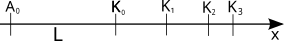
\includegraphics{Achilles.png}
\end{center}
\begin{itemize}
	\item カメは、アキレス$(A_0)$よりも$L$だけ前方$(K_0)$からスタートする。
  \item アキレスが$K_0$に到達するまでに、カメは$K_1$まで進んでいる。
  \item アキレスが$K_1$に到達するまでに、カメは$K_2$まで進んでいる。
  \item アキレスが$K_2$に到達するまでに、カメは$K_3$まで進んでいる。
  \item $\vdots$
  \item (以降、これをどれだけ繰り返しても、アキレスは、永久にカメに追いつくことはできない。)
\end{itemize}
これが、ゼノンの唱えた「アキレスとカメのパラドックス」と呼ばれるものである。

当然、現実には、アキレスはカメに追いつき、追い越すことが可能なはずであるが、
この論理によるとそれが不可能であることになる。
つまり、これは、一種の逆説(パラドックス)となっているのである。

\newpage

\section{定量的考察}

\subsection{具体的に考える}

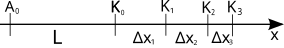
\includegraphics{AchillesDiff.png}

\begin{itemize}
  \item $L$ $\dots$アキレスとカメの初めの距離
  \item $v_A$ $\dots$アキレスの走る速度
  \item $v_K$ $\dots$カメの歩く速度
\end{itemize}
とする。

\subsubsection{第1段階}
アキレスが$K_0$に到達するのにかかる時間を$t_1$とすると、

$t_1$は$L$を$v_A$で割った値になるから、
\begin{displaymath}
  t_1 = L / v_A
\end{displaymath}
その間にカメが移動する距離を$\varDelta x_1$とすると、

$\varDelta x_1$は$v_K$に$t_1$をかけた値になるから、
\begin{eqnarray*}
  \varDelta x_1 &=& v_K \centerdot t_1 \\
                &=& L\left( \frac{v_K}{v_A} \right)
\end{eqnarray*}

\subsubsection{第2段階}
アキレスが$K_1$に到達するのにかかる時間を$t_2$とすると、

$t_2$は$\varDelta x_1$を$v_A$で割った値になるから、
\begin{eqnarray*}
  t_2 &=& \varDelta x_1 / v_A \notag \\
      &=& L\left( \frac{v_K}{v_A} \right)\frac{1}{v_A} \notag \\
      &=& \frac{L}{v_A}\left( \frac{v_K}{v_A} \right)
\end{eqnarray*}
この間にカメが移動する距離を$\varDelta x_2$とすると、

$\varDelta x_2$は$v_K$に$t_2$をかけた値になるから、
\begin{eqnarray*}
  \varDelta x_2 &=& v_K \centerdot t_2 \\
                &=& v_K\frac{L}{v_A}\left( \frac{v_K}{v_A} \right) \\
                &=& L\left( \frac{v_K}{v_A} \right)^2
\end{eqnarray*}

\subsubsection{第3段階}
アキレスが$K_2$に到達するのにかかる時間を$t_3$とすると、

$t_3$は$\varDelta x_2$を$v_A$で割った値になるから、
\begin{eqnarray*}
  t_3 &=& \varDelta x_2 / v_A \notag \\
      &=& L\left( \frac{v_K}{v_A} \right)^2 / v_A \notag \\
      &=& \frac{L}{v_A}\left( \frac{v_K}{v_A} \right)^2
\end{eqnarray*}
この間にカメが移動する距離を$\varDelta x_3$とすると、

$\varDelta x_3$は$v_K$に$t_3$をかけた値になるから、
\begin{eqnarray*}
  \varDelta x_3 &=& v_K \centerdot t_3 \\
                &=& v_K\frac{L}{v_A}\left( \frac{v_K}{v_A} \right)^2 \\
                &=& L\left( \frac{v_K}{v_A} \right)^3
\end{eqnarray*}

\subsubsection{第n段階}
$(1),(2),(3)$から、第n段階について、一般に、
\begin{equation}
  t_n = \frac{L}{v_A}\left( \frac{v_K}{v_A} \right)^{n-1} \tag{$*$}
\end{equation}
が推測される。

\newpage

\subsection{(*)の推測の証明}
(*)の推測
\begin{equation}
  t_n = \frac{L}{v_A}\left( \frac{v_K}{v_A} \right)^{n-1} \tag{$*$}
\end{equation}
ここからは、これがすべての自然数$n$について成立することを証明していく。

(証明)

数学的帰納法を用いる。
\begin{itemize}
\item $n = 1$のとき
\begin{eqnarray*}
   t_1 = \frac{L}{v_A} = \frac{L}{v_A}\left( \frac{v_K}{v_A} \right)^0
\end{eqnarray*}
これは、(*)に一致する。よって、(*)は成立する。

\item $n = k$のとき、(*)が成立すると仮定すると、
  \begin{displaymath}
    t_k = \frac{L}{v_A}\left( \frac{v_K}{v_A} \right)^{k-1}
  \end{displaymath}
  従って、$\varDelta x_{k+1}$は$v_K$に$t_k$をかけた値になるから、
\begin{eqnarray*}
  \varDelta x_{k+1} &=& v_K \centerdot t_k \notag \\
                    &=& v_K \frac{L}{v_A}\left( \frac{v_K}{v_A} \right)^{k-1} \notag
\end{eqnarray*}
    よって、$t_{k+1}$は$\varDelta x_{k+1}$を$v_A$で割った値になるから、
\begin{eqnarray*}
  t_{k+1} &=& \varDelta x_{k+1} / v_A \notag \\
          &=& v_K\frac{L}{v_A}\left( \frac{v_K}{v_A} \right)^{k-1} / {v_A}  \notag \\
          &=& \frac{L}{v_A}\left( \frac{v_K}{v_A} \right)^{k} \\
          &=& \frac{L}{v_A}\left( \frac{v_K}{v_A} \right)^{(k+1)-1}
\end{eqnarray*}
よって、$n = k+1$について、(*)が成立する。
\end{itemize}
以上から、数学的帰納法により、
\begin{displaymath}
  t_n = \frac{L}{v_A}\left( \frac{v_K}{v_A} \right)^{n-1} \tag{$*$}
\end{displaymath}
が全ての自然数$n$について成立することが示された。\hspace{\fill}Q.E.D
%\begin{flushright}
%Q.E.D
%\end{flushright}

\newpage

\section{パラドックスの解決}
各段階でかかる時間$t_n$は
\begin{displaymath}
  t_n = \frac{L}{v_A}\left( \frac{v_K}{v_A} \right)^{n-1} \tag{$*$}
\end{displaymath}
であることは、先に示した。

次に、$t_n$の第1項から第n項までの総和$S_n$を求めてみる。

これは、すなわち第$n$段階までの試行に必要な時間の総和を求めることを意味する。

$t_n$は、初項:$L/v_A$ 公比:$v_K/v_A$の等比数列である。

従って、その総和$S_n$は、付録にある、
初項$a$、項比$r$の数列の総和の公式より、
\begin{displaymath}
  S_n = a\frac{1-r^{n+1}}{1-r} \tag{$**$}
\end{displaymath}
であるから、
\begin{eqnarray*}
  S_n &=& \frac{L}{v_A}\frac{1-(v_K/v_A)^{n+1}}{1-(v_K/v_A)} \\
      &=& L\frac{1-(v_K/v_A)^{n+1}}{v_A-v_K}
\end{eqnarray*}
となる。ここで、$v_A > v_K$のとき、$n\rightarrow \infty$とすると、
\begin{eqnarray*}
  S = \lim_{n\to \infty}S_n &=& \lim_{n\to \infty}L\frac{1-(v_K/v_A)^{n+1}}{v_A-v_K} \\
                        &=& \frac{L}{v_A - v_K}
\end{eqnarray*}
よって、無限階段の試行を行うのに要する時間の総和$S$は、無限大ではなく、
\begin{displaymath}
  S = \frac{L}{v_A - v_K}
\end{displaymath}
という有限の値に収束する。

したがって、アキレスは、有限な時間でカメに追いつくことが可能である。
そして、追いつくのに要する時間は、初期の距離$L$を、二者の速度差$v_A-v_K$で割ったものと等しくなる。
これは、普通に計算した場合の値と、ぴたりと一致する。

\section{ゼノンの落とし穴}

では、ゼノンのパラドックスは一体どこに落とし穴があったのであろうか?
それは、一言でいえば、「無限」の扱いに不備があると言える。

「無限回の試行には、必ず、無限大の時間が必要である。」これが、間違いの元凶である。
この場合、試行の回数が増えるにつれて、足し合わせる値$t_n$はどんどん小さくなっていくのである。
そして、最終的には、ゼロに限りなく近づいてしまう。従って、$t_n$を無限回足しこんでも、
その値は、無限大には発散せず、有限の値に収束するのである。

\newpage

\section{※付録}
\subsection{等比級数の総和}
初項:$a$、公比:$r$の等比数列$a_n$
\begin{displaymath}
  a,ar,ar^2,ar^3,ar^4,ar^5,\dots,ar^n
\end{displaymath}
を考える。

これの第1項から、第n項までの総和$S_n$を求める。すなわち、
\begin{equation}
  S_n = a + ar + ar^2 + ar^3 + ar^4 + \dots + ar^n \tag{1}
\end{equation}
ここで、$r \times S_n$を考えると、
\begin{equation}
  rS_n = ar + ar^2 + ar^3 + ar^4 + ar^5 + \dots + ar^{n+1} \tag{2}
\end{equation}
となり、各項が一つずつずれる。
そして、$(1) - (2)$を行うと、

\begin{tabular}{lllll}
           &$S_n$   &= $a$ &$+ ar + ar^2 + ar^3 + ar^4 + \dots + ar^n$ &\\
       $-)$&$rS_n$  &=     &$+ ar + ar^2 + ar^3 + ar^4 + \dots + ar^n +$ &$ar^{n+1}$ \\ \hline
    $(1-r)$&$S_n$   &= $a$ &                                             &$ - ar^{n+1}$
\end{tabular}

と、最初の項と最後の項以外が、全て消えることになる。

よって、$r \neq 1$のとき、両辺を$1 - r$で割って、
\begin{align}
  S_n &= \frac{a - ar^{n+1}}{1-r} \notag \\
      &= a\frac{1-r^{n+1}}{1-r} \tag{$**$}
\end{align}
が得られる。\par

ちなみに、$r = 1$のときは、数列$a_n$は、
\begin{equation}
  a, a, a, a, a, \dots ,a \notag
\end{equation}
となるので、これの第$1$項から第$n$項までの総和$S_n$は、
\begin{equation}
  S_n = an \notag
\end{equation}
となる。

\end{document}
